\documentclass{article}

\usepackage[utf8]{inputenc} 
\usepackage{outlines}
\usepackage{amsmath}
\usepackage{cleveref}
\usepackage{xr}
\usepackage{siunitx}
\usepackage{multirow}

\usepackage{natbib}
\bibliographystyle{abbrvnat}

\usepackage[margin=1in]{geometry}
\parskip 1.5ex % paragraph spacing

\usepackage{graphicx}
\graphicspath{./docs/Figures/}

\title{Variation in thermal sensitivity of ecological traits drives patterns of species richness across temperature gradients}
\author{Tom Clegg, Samraat Pawar}
\date{January 2021}

\begin{document}

\maketitle

\section*{Abstract}

...

\section*{Introduction}

The effect of temperature on biodiversity has long been a topic of interest in ecology \citep{Gaston2000}. Starting with the pioneering work of Alexander von Humboldt who in the 19th century identified temperature as a major environmental driver of plant richness along elevational gradients in the Andes (REF), many relationships between taxonomic richness and temperature have been identified across different taxa and environments with various mechanisms being suggested to explain these patterns \citep{Rohde1992,Gaston2000}. In recent years the response of richness in microbial communities to temperature has become a topic of particular interest as awareness of their importance in maintaining the key ecosystem functions increases (REF) and new sequencing technologies allow whole microbial communities to be characterised with relative ease (REF).  

Broadly the effects of temperature on microbial communities are well documented, with many studies showing how temperature affects their structure (REF), function (REF) and patterns of diversity (REF). Broadly, this temperature dependence can be explained by the dependence of these properties on individual metabolic rate which determines the capacity of individuals to grow and interact with their external environment. The temperature dependence of metabolic rate is in turn determined by biochemical kinetics which are predictable, thus providing way to understand and predict the responses of emergent properties of interest \cite{Gillooly2001,Brown2004}. 

Though some consistencies in the thermal responses of microbial communities exist (REF), studies looking specifically at richness have generally found mixed responses to temperature which depend on the specific system being considered. For example, whilst REF found that soil microbe richness increased across a continental temperature gradient in North America others have found unimodal responses in tropical oceans (REF) and geothermal environments (REF), with richness peaking at intermediate temperatures. This variation in the temperature-richness relationship was further demonstrated and quantified in a meta-analysis by REF which showed that large variation in the temperature responses of microbial richness exists and that no single pattern (i.e shape or direction) dominates the temperature response in soil microbe communities. 

Unsurprisingly the presence of such variation has resulted in several mechanisms being suggested to explain the richness-temperature relationship in microbial communities. The metabolic theory of biodiversity (MTB) predicts that richness should increase with temperature based on the assumption of energy equivalence of populations (REF), with the log of richness following a linear relationship when plotted against the inverse of temperature (REF). This prediction is centered around the assumption of a single global temperature dependence across all taxa but has been met with limited support in microbial systems (REF). Another mechanism that has been suggested to explain the thermal response of microbial diversity is the metabolic niche hypothesis (REF), that at intermediate (non-extreme) temperatures there are more energetically viable ways to make a living, allowing greater potential diversity (REF). Although some observations of microbial richness appear to follow this predicted unimodal relationship (REF), it is by no means a universal rule. 

Whilst these mechanisms have provided some insight into how microbial richness responds to temperature one aspect that has not been considered is the variation that exists in the thermal responses between and within different microbial taxa (REF). This variation has been highlighted by a number of studies using both meta-analyses and experimental approaches (REF), demonstrating how the temperature responses of key metabolic traits such as growth and respiration consistently varies between microbial taxa (REF). This variation is expected to be important in determining the responses of microbial communities to temperature through two mechanisms. Firstly, the non-linear nature of individual temperature responses means that variation in thermal response parameters across taxa will have significant effects on the distributions of metabolic traits across taxa at different temperatures \citep{Savage2004}. This in turn will affect the response of community dynamics  to temperature and thus emergent properties such as richness. The potential impact of this variation becomes especially important when we consider the additional complexity of the non-linear interactions that have been shown to be important in microbial communities (REF), which may serve to amplify these effects. Secondly, variation in thermal responses will create ``thermal mismatches`` between different populations and traits which can result in altered responses to temperature at the community level (REF). This occurs as differences in thermal responses between taxa or traits result in changes to the relative trait values of populations or specific traits across temperature, resulting in shifts in community dynamics and thus emergent properties such as richness. Such effects have already been demonstrated in various ecological contexts including predator-prey (REF) and virus-host (REF) systems and will likely be important in microbial systems given the significant variation in thermal responses that  exists. 

In this paper we investigate the effect of this variation in thermal sensitivity in driving patterns of richness of microbial communities across temperature. Using a general model of community dynamics we first derive analytical results, explicitly linking variation in thermal sensitivity to the number of populations that can coexist within a community. In doing so we account for the effects of variation on both the distributions of traits within ecosystems and in the mismatches between different metabolic traits. Then, using a newly-assembled data set of prokaryotic growth curves, we parameterise the model to show that realistic estimates of variation in thermal sensitivity are relevant in driving patterns of richness across temperature in microbial communities. Finally we show that our analytical results are robust to relaxations of our assumptions in the analytical model using numerical simulations of complex species-rich communities. 

\section*{Methods}

\subsection*{Theory}

Our overall approach is to first link the effects of a given distribution of key traits (i.e., growth rates and interaction strengths) to feasibility: the capacity for a community to support all populations (i.e., maintain non-zero biomass) at equilibrium  \citep{Grilli2017,Dougoud2018}. Feasibility is a necessary condition for stable population coexistence and by deriving an expression for feasibility we are able to determine the maximum richness a system will be able to support given their specific trait values. We then go on to determine the effects of temperature on this relationship and finally use numerical simulations of assembly in complex, species-rich ecosystems to test our analytical approximations. 

\subsubsection*{Model}
In order to quantify the effects of temperature on feasibility and richness, we use the generalised Lotka-Volterra model (GLV) of an $N$ species community, with the growth of the $i$th species given by
\begin{equation} \label{EQ:GLVM}
  \frac{1}{x_i} \frac{dx_i}{dt} = r_i(T) - \sum^N_{j = 0} a_{ij}(T) x_j, 
\end{equation}
where $x_i$ is its biomass density ($\text{mass} \cdot \text{volume}^{-1}$), $r_i(T)$ it's intrinsic growth rate determining the rate at which new biomass is produced ($\text{time}^{-1}$), $a_{ij}(T)$ is the effect of interactions with the $j$th species' population (with $a_{ii(T)}$ representing the strength of of intraspecific interactions; $\text{volume} \cdot \text{mass}^{-1} \cdot \text{time}^{-1}$). Note that all the parameters are expressed as functions of temperature ($T$), the form of which will be addressed later. 

\subsubsection*{Feasibility and Species Richness} \label{SEC:Feas_SP_rich}

We next derive an expression to determine the feasibility of a community in terms of the parameters in \cref{EQ:GLVM} and species richness. Though we consider only feasibility here, previous work has shown that in GLV systems feasible fixed points are almost always stable (REF). Thus, if we want to determine how many populations will be able to persist in a given community it is sufficient to show that the maximum number of species a community may have and remain feasible. This will ensure that it is dynamically stable and that populations within will thus be able to persist. 

In order to determine the feasibility of a community we need to first derive an expression for equilibrium biomass, $x^*_i$. Though it is not possible to derive an exact analytical solution for the GLV (\cref{EQ:GLVM}), we use a mean-field approximation (\cref{SI_Sec:Meanfield};  \citet{Wilson2003,Wilson2004}), which allows us to derive an expression for equilibrium biomass in terms of the average effect of interactions ($\bar{a}$) across the community as: 
\begin{equation}\label{EQ:MF_equi}
  x^*_i \approx K_i(T) -  \bar{K}(T)  \frac{ (N-1)\bar{a}(T)}{1 + (N-1)\bar{a}(T)}. 
\end{equation}
Here, $K_i = \frac{r_i(T)}{a_{ii}(T)}$ is the $i$th species carrying capacity (the biomass this population would reach if grown in isolation, obtained by solving \cref{EQ:GLVM} with no interactions), $N$ is species richness, and $\bar{a}(T)$ and $\bar{K}(T)$ are the average pairwise, interspecific interaction strength and carrying capacity respectively. \Cref{EQ:MF_equi} provides an intuitive expression for equilibrium biomasses; a population will reach the biomass that it would in isolation (first term, $K_i(T)$) minus the effects of any interspecific interactions (second term). The strength of these interspecific interaction effects is determined by the average carrying capacity of all other species ($\bar{K}(T)$) and a saturating function of the interspecies interaction strength experienced by the focal species, $(N-1)\bar{a}(T)$. If interactions are overall competitive (i.e., $\bar{a}(T) > 0$) then equilibrium biomass will be reduced relative to the individual carrying capacities, and if they are facilitatory (i.e., cooperative or mutualistic; $ \bar{a}(T) < 0$), it will increase. This approximation (\cref{EQ:MF_equi}) relies on the assumption that the system is large (large number of species) and that no individual pairwise interaction dominates. We test the sensitivity of our results to these key assumptions later using numerical simulations.

Next we use \Cref{EQ:MF_equi} to derive an expression for community feasibility in terms of the population-level traits (i.e., the $r(T)$'s and $a(T)$'s) which will then be used to determine the upper bound on species richness $N$. An ecosystem is feasible if all species have non-zero equilibrium biomasses (i.e., $x_i^* > 0 $), a condition that can be expressed as:
\begin{align} \label{EQ:Feas_sp}
  \kappa_i(T) > \frac{(N-1)\bar{a}(T)}{1 + (N-1)\bar{a}(T)} \quad \text{for all} \quad i = 1 \ldots N.
\end{align}
Here, $\kappa_i = \frac{K_i(T)}{\bar{K}(T)}$ is the mean-normalised carrying capacity of the $i$th species. \Cref{EQ:Feas_sp} shows that an ecosystem is feasible as long as the the effects of interspecific interactions on each population (RHS) do not outweigh it's mean normalised carrying capacity (LHS). If interactions are competitive ($\bar{a}(T) > 0$) and strong, the inequality will not hold, extinctions will occur and the system will be unfeasible. If interactions are on average facilitatory ($\bar{a}(T) < 0$) then the LHS will always be negative and the inequality will hold as by definition $\kappa > 0$. 

Using \cref{EQ:Feas_sp} we next derive an expression for $P_{feas}$, the probability that a community is feasible given the distribution of species trait values ($\kappa$s and $a$s) and number of species ($N$) in the system. To do so we take \cref{EQ:Feas_sp} and consider $\kappa$ and $a$ as random variables, each describing the distribution of the respective traits across the populations in the community (denoted by the loss of subscript). This allows us to consider $\kappa$'s cumulative density function (CDF), i.e., the probability that it is less than or equal to some value: $F_{\kappa}(x,T) = P(\kappa \leq x)$. As the condition for feasibility states that $\kappa$ must be greater than the effect of interactions we can use this CDF and the condition in \cref{EQ:Feas_sp} to express $P_{feas}$ as
\begin{equation} \label{EQ:P_feas}
    P_{feas} = P \left( \kappa(T) > \frac{(N-1)\bar{a}(T)}{1 + (N-1)\bar{a}(T)}  \right)^N = 
    \left[1 - F_{\kappa}\left(\frac{(N-1)\bar{a}(T)}{1 + (N-1)\bar{a}(T)},T \right)\right]^N,
\end{equation}
giving the probability of feasibility of an ecosystem as a function of the species traits. Note the expression is raised to the $N^\text{th}$ power because the term in the brackets must hold for all $N$ populations in a community for it to be feasible. \Cref{EQ:P_feas} makes explicit the effect of species richness $N$ on the probability of feasibility in a community, showing how $P_{feas}$ will decline with increasing $N$ through two mechanisms. Firstly it alters the strength of interactions experienced by individual populations via the $(N-1) \bar{a}(T)$ term. A higher species richness means that the strength of interactions will be greater and if interactions are on average competitive ($\bar{a}(T) > 0$) this will reduce the chance the condition in \cref{EQ:P_feas} is met, reducing the probability of feasibility. Secondly, the probability of feasibility will fall as the number of species increases as it becomes less likely that all $N$ species meet the criteria in \cref{EQ:Feas_sp} as represented by the $N\text{th}$ power term in \cref{EQ:P_feas}. 

Importantly, this decline in $P_{feas}$ with increasing richness places an upper bound on species richness given a certain distribution of $\kappa$ and $a$ values within a community. If a system is too large then we expect that it will have a low probability of feasibility and thus be likely to experience population extinctions until the probability of feasibility becomes larger and extinctions become unlikely. Although ideally we would use \cref{EQ:P_feas} to determine this bound explicitly by solving for $N$ this is not possible for most distributions of $\kappa$ due to the complexity of their CDFs. We therefore use a numerical approach to determine the exact value of this upper bound on $N$ (see SI). It is important to note that this does not preclude insights into the effects of variation in thermal sensitivity which we now address. 

\subsubsection*{Temperature responses of traits} \label{SEC:Temperature}
Having defined the relationship between species richness and the distribution of species' traits across the community, we now turn to the effect of temperature. Broadly, our approach here is to consider how the distributions of the relevant species traits across populations change with temperature and thus $P_{feas}$ and the upper bound on $N$. We derive expressions for these trait distributions in terms of the distributions of their thermal sensitivity. This allows us to quantify the effect of variation in thermal sensitivity between species' populations as well as traits on the temperature-species richness relationship. We use the Boltzmann-Arrhenius equation to represent the temperature dependence of $\kappa$ and $a$ (Savage 2004 am nat):
\begin{equation} \label{EQ:Boltzmann}
    B(T) = B_0 e^{-\frac{E}{k} \left(\frac{1}{kT} - \frac{1}{k T_{ref} }\right)}.
\end{equation}
Here, $B(T)$ is the relevant trait value,  $T$ is temperature in Kelvin, $B_0$ is the normalisation constant, i.e., the trait value at some reference temperature ($T_{ref}$, also in Kelvin), $E$ (eV) is the thermal sensitivity which determines the change in trait value to a unit change of $\frac{1}{kT}$, and $k$ is the Boltzmann constant. Although empirically-measured thermal performance curves of single individuals or species are generally unimodal, the Boltzmann-Arrhenius equation adequately captures the the rising portion (before the temperature peak) of these curves, which is also the temperature range within which individuals and populations typically operate (or experience) (the ``Operational Temperature Range'', or OTR) \cite{Dell2011}. Thus focusing on the Boltzmann-Arrhenius portion of thermal performance curves is relevant to the dynamics of real ecosystems, and also, conveniently, affords us analytic tractability . 

Applying \cref{EQ:Boltzmann} allows us to characterise the distributions of parameters across species populations at different temperatures in terms of the distributions of the underlying parameters $B_0$ and $E$. Assuming that the trait value, $B(T)$, follows a log-normal distribution across the community we let $\log(B_0)$ and $E$ follow normal distributions, allowing us to obtain an explicit expression for the temperature dependent distribution of $B(T)$ (see \cref{SI_Sec:TPC_dist}):
\begin{align} \label{EQ:Boltz_dist}
    \log(B(T)) \sim \mathcal{N}\left(\mu_{B}(T) , \sigma_{B}^2(T) \right) 
    \quad \text{where} \quad
    \begin{array}{cc}
        \mu_B(T) &= \mu_{B_0} - \mu_{E} \left(\frac{1}{kT} - \frac{1}{k T_{ref} }\right)  \\
        \sigma_{B}(T)^2 &= \sigma_{B_0}^2 + \sigma_{E}^2 \left(\frac{1}{kT} - \frac{1}{k T_{ref} }\right)^2 .
    \end{array}
\end{align}
Here, $\log(B_0)$ and $E$ are both normally distributed, with $\mu$ and $\sigma$ denoting their mean and standard deviations respectively. \Cref{EQ:Boltz_dist} makes explicit the effect of the distribution of thermal response parameters on the distribution of $B(T)$, showing how both $\mu_B(T)$ and $\sigma_B(T)$ are functions of temperature. In both cases the parameters determining the distribution of $B_0$ act as constants, with the strength and nature of the temperature response being solely determined by the distribution of $E$ values. The average thermal sensitivity $\mu_E$ determines the strength of the relationship thermal response of $\mu_B(T)$ as a linear function whilst $\sigma_E$ determines the thermal response of $\sigma_B(T)$ as a quadratic. It is important to note that as $B(T)$ is log-normally distributed its moments are determined by both $\mu_B(T)$ and $\simga_B(T)$ and thus both temperature dependent factors (the linear and quadratic parts) will determine it's distribution in linear scale.

Applying \cref{EQ:Boltz_dist} to the distributions of $\kappa$ and $\bar{a}$ we obtain the expressions
\begin{align} 
        \log(\kappa(T)) &\sim \mathcal{N}\left( -\frac{\sigma_{K}^2(T)}{2} , \sigma_{K}^2(T) \right) \quad \text{and} \label{EQ:Trait_distributions_K} \\ \nonumber \\
        \bar{a}(T) &= \exp \left(\mu_a(T) + \frac{\sigma_a^2(T))}{2} \right) \label{EQ:Trait_distributions_a},
\end{align}
which show how the temperature responses of $\kappa$ and $\bar{a}$ are determined by their respective thermal response parameter distributions. \Cref{EQ:Trait_distributions_K,EQ:Trait_distributions_a} show that distribution of $\kappa$ is is independent of the mean term $\mu_{K}(T)$, being fully determined by the variance term $\sigma_{K}^2(T)$ whilst $\bar{a}$ is determined by both the average $\mu_a(T)$ and variance $\sigma_a^2(T)$ terms. This means that moments defining the distribution of $\kappa$ will include only the quadratic temperature terms, the strength of which is determined by the variation in thermal sensitivity $\sigma_{E_{\kappa}}$. $\bar{a}$ will also include the linear temperature term the strength of which is determined by the average thermal sensitivity, $\mu_{E_a}$. 

Combining \cref{EQ:Trait_distributions_K,EQ:Trait_distributions_a} with the equation defining $P_{feas}$, \cref{EQ:P_feas}, provides important insight into the effect of the distribution of thermal parameters on the thermal response of species richness. The overall direction and magnitude of the richness-temperature relationship will be determined by the average thermal sensitivity of interactions $\mu_{E_a}$, with richness following the inverse temperature dependence of interaction strength (as stronger competitive interactions result in lower richness as per \cref{EQ:P_feas}). The variation in thermal sensitivity, $\sigma_{E_a}$ and $\sigma_{E_{\kappa}}$ will determine the relative strength of the quadratic term in the richness temperature relationship and only when variation is large enough will it be large enough to introduce curvature in the richness temperature response.


\subsection*{Calculating the thermal response curves of Species Richness} \label{SEC:Temp_SP_num}

In order to obtain quantitative predictions of the effect of temperature on species richness from the analytic expressions above, we substitute \cref{EQ:Trait_distributions_K,,EQ:Trait_distributions_a} into the expression for $P_{feas}$ (\cref{EQ:P_feas}), and solve for $N$. Whilst ideally this would be done analytically, the complexity of the CDF for the distribution of $\kappa$ prevents such an approach and we instead solve for $N$ numerically. To this end, we set a lower threshold value of $P_{feas}$, $\theta$, as well as values for the parameters controlling the distributions of the thermal responses for both $a$ and $\kappa$. We then use golden-section search optimisation to search for the maximum value of $N$ with the given $\theta$ value \citep{Mogensen2018}. Repeating this procedure at different temperatures gives the full temperature richness curve for any given set of parameters. We calculated such species richness - Temperature curves for different combinations of means and variances of thermal sensitivity of $K$ and $a$. Holding either $\kappa$ or $a$'s distributions constant, we calculated species richness curves in a fully factorial manner setting ($\mu_{E} \in [-0.65, 0.0, 0.65]$ and $\sigma_{E} \in [0.0, 0.5, 1.0]$). We did not vary the average thermal sensitivity of $K$ as \cref{EQ:Trait_distributions_K} shows the realised distribution of $\kappa$ is independent of the average value. We also fix the distribution of normalisation constants, using the empirical distributions discussed bellow for $\kappa$ and setting $\mu_{a_0} = -2$ and $\sigma_{a_0} = 0.5$.

\subsection*{Data}

To explore the relevance of variation in thermal sensitivity on species richness, we compiled a new data set of prokaryotic population growth curves at different temperatures to obtain realistic estimates of the distributions of thermal response parameters across species. We then use this empirical distribution to parameterise our analytical expression for feasibilit and calculate the resultant species richness temperature response to explore the effects of reallistic levels of variation in thermal resposnes. 

Our dataset was constructed by digitising 875 individual growth curves (i.e., measurements of biomass/population size over time) representing 224 species/media combinations for which we have measurements over multiple temperatures. These growth curves were spread across 105 strains from 21 separate studies. We then fit the logistic growth model to each of these individual growth curves using non-linear least squares, giving us estimates of carrying capacity across multiple temperatures for each unique strain-media combination. After filtering for fits that did not converge, were non-significant ($p > 0.05$) or had measurements across less than three unique temperatures, we were left with 73 unique sets of estimates for carrying capacity $K$ across temperature. We then fit the Boltzmann-Arrhenius and Sharpe-Schoolfield \citep{Schoolfield1981} to each of these sets in order to account for cases where $K$ displayed peaked or non-peaked thermal responses, selecting the best fitting model for each temperature curve using AIC. After removing measurements for which no model converged we were left with 74 estimates of thermal response parameters for $K$. From these data we obtained the mean and variance for the normalisation constant $\log(K_0)$ and thermal sensitivity $E_K$ by fitting a normal distribution using maximum-likelihood estimation (MLE) (REF). In order to assess the effect of including the observed variation in thermal sensitivity we plot the species richness temperature curve in two scenarios, one with the variation in thermal sensitivity observed in our data and one where variation is set to $0$ and all species share the same universal thermal sensitivity value. 

\subsection*{Community assembly simulations}

Finally, in order to test the bound on species richness and the effects of temperature we simulate the assembly of communities using the full GLV in \cref{EQ:GLVM}. This allows us to test the generality of the analytical predictions for the species richness by relaxing the assumptions made by the mean-field approximation about ecosystem dynamics. We use assembly here as a way to allow systems to reach the maximum species richness (i.e., the prediction generated by the model) given the distributions of thermal sensitivity parameters and temperature. 

To simulate assembly we start with an empty system at a given temperature which we assemble into a community through sequential species invasions. Each invader has thermal performance traits ($B_0$s and $E$s) drawn from a global distribution which are used to calculate the actual trait values ($\kappa$s and $a$s) at that temperature. Following each invasion we simulate the system till it reaches steady state, remove extinct populations and record the species richness. At each time step we calculate the coefficient of variation $\text{CV} = \frac{\mu}{\sigma}$ of richness over the last $50$ immigration events, giving a measure of the variation of species richness over time. We stop the simulations when the coefficient of variance is smaller than some lower threshold $\text{CV} < 0.05$, indicating that richness has reached quasi-equilibrium and is constant over time. This process is then repeated at different temperatures using the parameterisations in \cref{Tab:SimParams} across different levels of variation in thermal sensitivity $\sigma_E \in [0.0, 0.25, 0.5]$, allowing us to examine the simulated temperature-species richness curves. All simulations were carried out using the Julia programming language and the DifferentialEquations.jl Package for numerical integration \citep{Rackauckas2017}. To assess the fit of the analytical predictions we use the approach detailed above, calculating predicted species richness given the global thermal trait distributions by setting lower threshold probability of feasibility $(\theta = 0.5)$ and solving for the maximum richness permitted at this threshold.

\begin{table}[h]
    \centering
   \begin{tabular}{llll}
        \hline
        \multicolumn{2}{l}{Parameter} & $\mu$        & $\sigma$          \\ \hline
        \multirow{2}{*}{$K$}  & $K_0$ & -0.14 *      & 0.58 *            \\
                              & $E_K$ & 0.05. *      & $[0.0, 0.5, 1.0]$ \\
        \multirow{2}{*}{$a$}  & $a_0$ & $\log(0.01)$ & $0.5$             \\
                              & $E_a$ & $-0.65$      & $[0.0, 0.5, 1.0]$ \\
        \hline
\end{tabular}
    \caption{\textbf{Parameters used for assembly simulations}. Values with indicate the parameter is from the empirical data set.}
    \label{Tab:SimParams}
\end{table}


\section*{Results}

\subsection*{The distribution of thermal sensitivities determines the thermal response of species richness}

We first examined the effect of the distribution of thermal sensitivities across populations on the temperature response of species richness. Overall both the mean and variance of thermal sensitivity distributions, $\mu_E$ and $\sigma_E$, had the expected effects on the species richness temperature relationship \cref{Fig:N_vs_T}. For $E_a$ the mean thermal sensitivity determined the overall direction of the thermal response (with richness following the inverse temperature dependence of interactions) whilst increasing variation lead to unimodality in the temperature response \cref{Fig:N_vs_T}a. Altering the variation in $E_{\kappa}$ also had the expected effect, introducing unimodality in the richness temperature response \cref{Fig:N_vs_T}b. 

\begin{figure}[h!] 
    \centering
    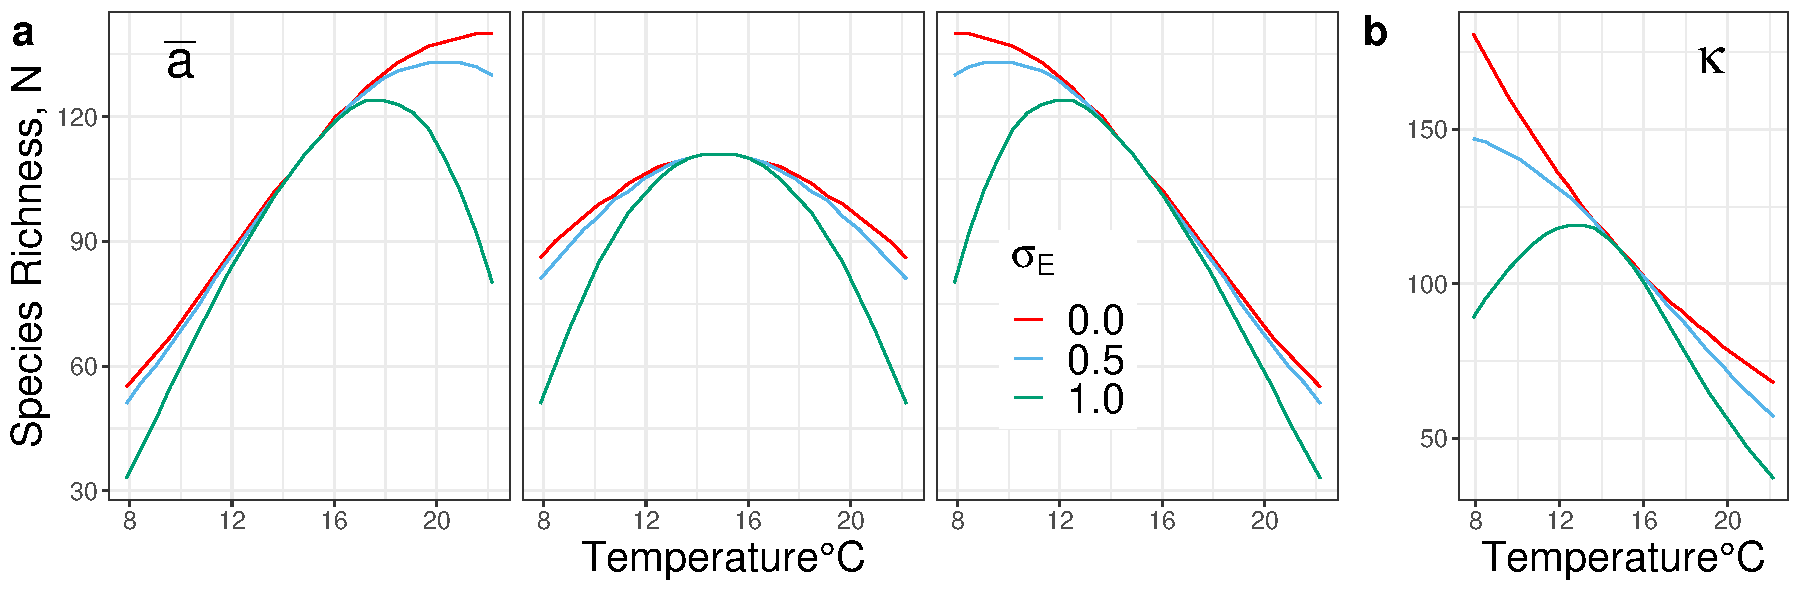
\includegraphics[width=0.8\textwidth]{docs/Figures/Fig_N_ana.pdf} 
    \caption{\textbf{The thermal response of species richness  varies with the distribution of thermal sensitives} a) The shape of distribution of thermal sensitivities of interactions $E_a$ alters the richness-temperature relationship. As predicted by \cref{EQ:Boltz_dist} the average thermal sensitivity (as shown in each panel) determines the overall direction of the thermal response whilst variance in thermal sensitivity (coloured lines, see legend) introduces additional curvature to the species richness response. b) Altering the variation in the thermal sensitivity of $\kappa$ has the same effect, creating curvature in  the species richness response (colored lines). Curves were generated using the approach outlined in methods with parameters $\sigma{\log(K_0)} = 0.5$, $\sigma_{E_K} = 0.2$, $\mu_{a_0} = log(0.01)$ and  $\sigma_{a_0} = 0.5$}
    \label{Fig:N_vs_T}
\end{figure}


\subsection*{Empirical variation in thermal sensitivity is relevant for community level thermal responses}

Our empirical dataset on the thermal performance of microbial growth showed significant variation in the thermal sensitivity of $K$ (\cref{Fig:TPC_data}). Normal distribution fits using maximum likelihood estimation yielded estimates of $\log(K_0) \sim \mathcal{N}(-0.14,0.58)$ and $E_K \sim \mathcal{N}(0.06,0.29)$ for the normalisation constant and sensitivity respectively (\cref{Fig:TPC_data}a-b). As expected, this empirically observed variation in the thermal sensitivity resulted in a unimodal response of species richness to temperature whilst the no-variation scenario resulted in a simple monotonic response (\cref{Fig:TPC_data}c). 

\begin{figure}[h!]
    \centering
    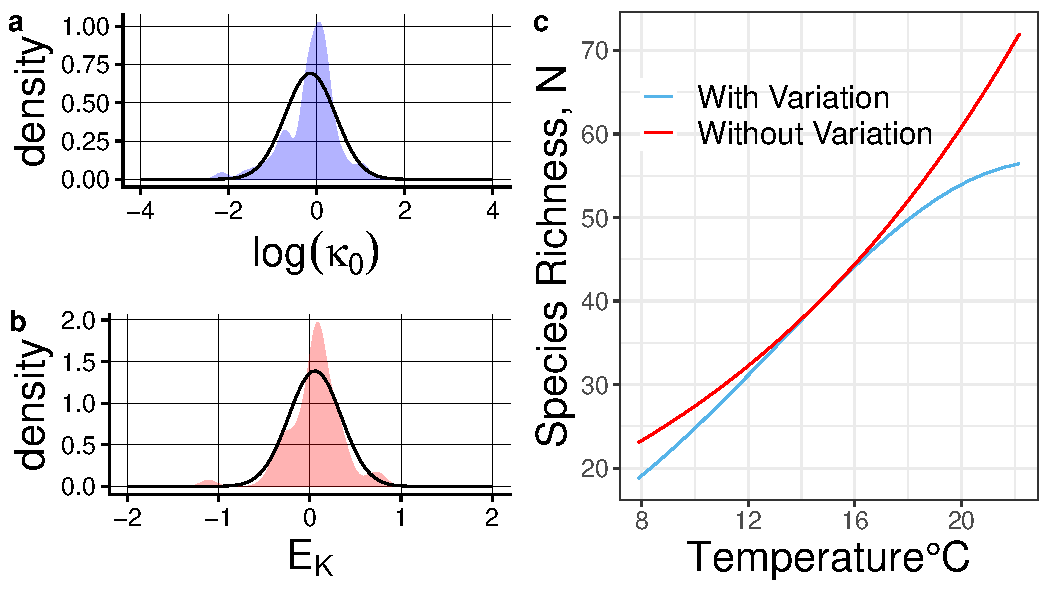
\includegraphics[width = 0.8\textwidth]{docs/Figures/MTE_fig.pdf}
    \caption{\textbf{Empirical variation in thermal sensitivity determines the thermal response of species richness }. a-b) Distributions of empirical estimates of a) $\log(K_0)$ and b) $E_K$. Colored density plots are the actual empirical distributions of the parameters with the solid black line showing the fitted normal distribution. The distribution of thermal sensitivity (b) demonstrates the existence of variation in the thermal response ($\sigma_{E_K} = 0.29$. c) Prediction of species richness thermal response using the empirical distributions. The blue and red lines represent the estimates with and without variance in thermal sensitivity, showing how the observed variance creates a unimodal response of species richness to temperature.}
    \label{Fig:TPC_data}
\end{figure}

\subsection*{The distribution of thermal sensitivities predicts the species richness of randomly assembled communities}

Our analytical result \cref{EQ:P_feas} was able to predict species richness patterns in randomly assembled communities across temperatures remarkably well (\cref{Fig:Temperature_assembly}). Across the randomly assembled communities, species richness followed the qualitative patterns expected from the analytical predictions, with the thermal response of richness exhibiting an increasingly unimodal shape with an increase in the variation in thermal sensitivity. The actual species richness reached by assembling communities matched the analytical predictions well, though the actual species richness reached by simulated communities deviated at the lower and higher ends of the temperature scale. 

\begin{figure}
    \centering
    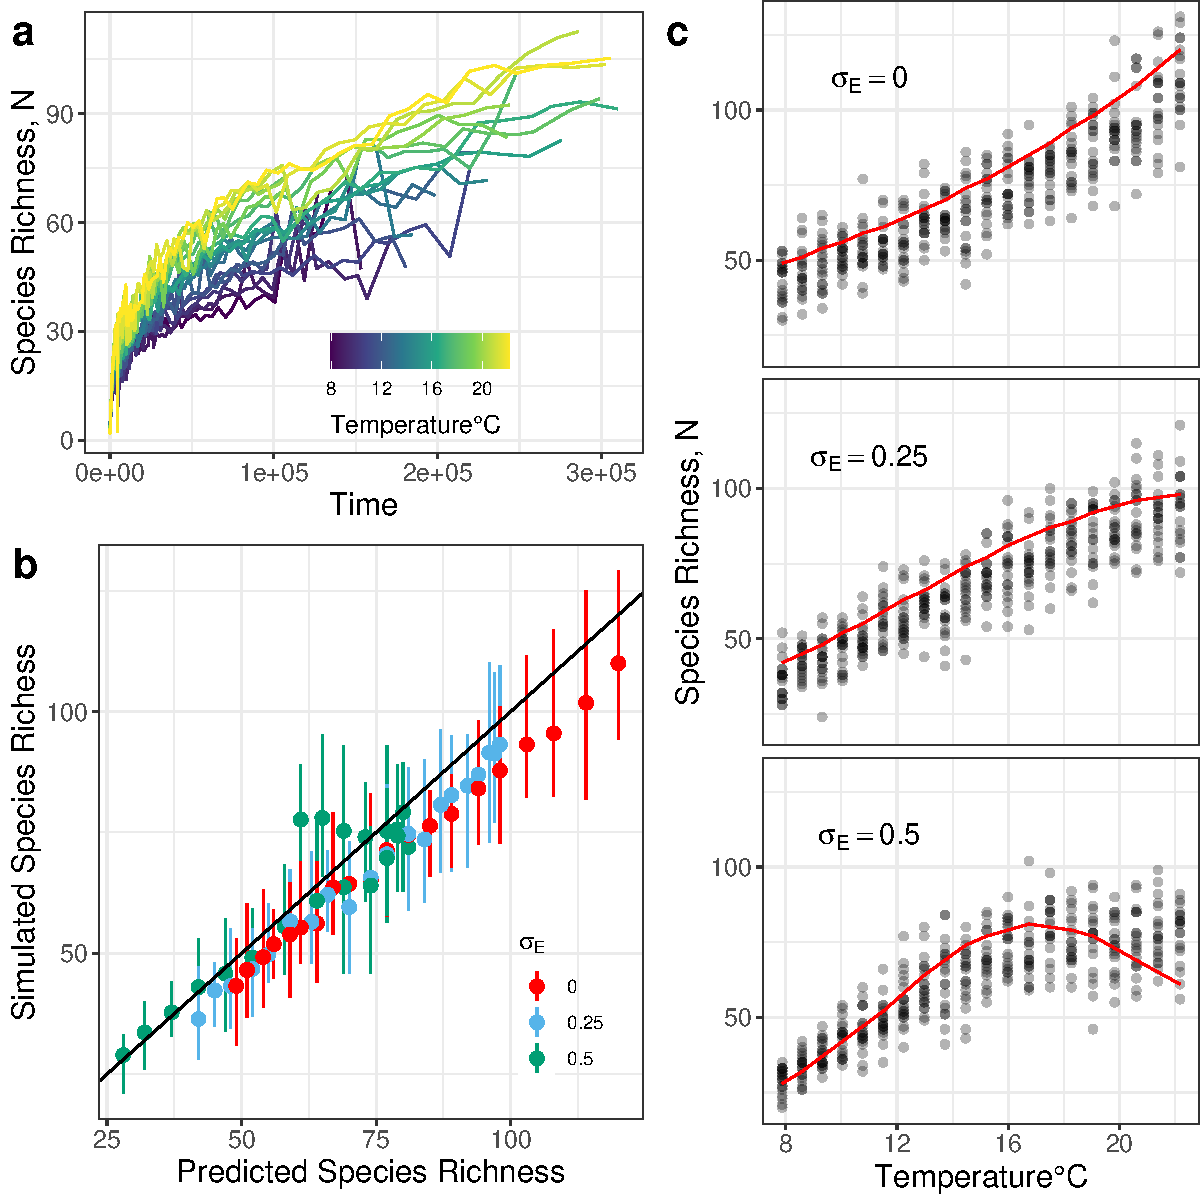
\includegraphics[width = 0.8\textwidth]{docs/Figures/Fig_sim.pdf}
    \caption{The assembly of ecosystems at different temperatures is predicted by the analytical feasibility condition. A) Trajectories of species richness over assembly across temperature at a single level of variation in $E$ ($\sigma_a = 0.25$). Each line is the average species richness over time at a given temperature. Species richness is seen to saturate over time, with systems assembling at higher temperatures having lower species richness. B) The observed final species richness reached by the assembly simulations plotted against the analytical predictions of \cref{EQ:P_feas}. Each point is the average species richness across the 5 replicates with error bars showing the standard deviation. The blue line and shaded region represent the 1:1 line of predictions and observations, representing a probability threshold of \SI{1e-10}, with the shaded region corresponding to the richness predicted by thresholds between \SI{1e-8}-\SI{1e-12}. . C-E) The species richness - temperature relationship at 3 levels of variation in $E$. Each points represents the species richness reached by a single assembly simulation with the red line and shaded area representing the predicted species richness at a threshold of \SI{1e-10} and within the bounds \SI{1e-8}-\SI{1e-12}. Overall the observed species richness and predictions match well with most observations falling within the prediction bounds. Only at the extremes of temperature (e.g. at 280K in (C)) do the observations significantly fall outside the prediction bounds.}
    \label{Fig:Temperature_assembly}
\end{figure}

\section*{Discussion}

Understanding how variation in thermal responses between different processes and taxa affects ecological communities is an important problem in ecology, especially given current rates of warming (REF). Here we show that through its effects on the distributions of key species traits, this variation affects the feasibility of ecosystems and thus the total species richness they can support. Furthermore, we have shown that the level of variation seen in a specific taxonomic group (bacteria) is sufficient to significantly affect this relationship and that the predictions of our analytical theory are robust to relaxation of key assumptions. 

Our analytical approach provides novel insights into the effects of the shape of the distribution of thermal sensitivity.  
    
    • Clearly our work shows the effect of altering the first two moments of this distribution
    
    • Our approach also makes this relationship explicit, avoiding the problem with simulation based methods such as \citet{Stegen2012} whose simulations are hard to gain general insight from

We use feasiblity as a mechanism to determine species richness 
    
    • This is one (importanat) ecosystem dynamics property which in and of itself does not grantee a system will persist
    
    • future work could extend the approach here with other properties such as stablity (though it is worth noting that feasbility implies stability in the GLV) and the newly developed extinction boundary (VAn's paper). 
    
Our results are robust to relaxations of the assumptions of the mean-field system
   
    • when we assemble communityies randomly their behaviour is  relatively well predicted
    
    • demonstrates that the analytical expectations should be applicable in a variety of contexts
    
    • Other models of ecosystem dynamics are possible, which may allow other types of systems to be explored in more detail (consumer resource, mutualisms?)

Our analysis of data on variation in thermal sensitvtiy shows that it is sufficent to affect the response of species richness curves.
    
    •   given that varation appears ubiquitous in nature this would imply that curved responses of richness with temperature should be more common
    
    •   Is in alignment with empirical data which shows the Temperature-Richness relationship is very variable

This work supports (growing?) focus on varation in thermal sensitbtiy as opposed to the use of a single universal value
    
    • important for other applications such as climate models?

\newpage

\bibliography{Temp_richness.bib}


\renewcommand{\thepage}{S\arabic{page}} 
\renewcommand{\thesection}{S\arabic{section}}  
\renewcommand{\thetable}{S\arabic{table}}  
\renewcommand{\thefigure}{S\arabic{figure}} 
\renewcommand{\figurename}{Supplemental Material, Figure} 

\setcounter{section}{0}

\section*{Supplementary Materials}

\subsection{Mean-field approximation} \label{SI_Sec:Meanfield}
In this section we show the derivation of the mean-field approximation and equilibrium solution. Broadly the mean-field approximation works by considering interactions through their average effect on species populations, not through their individual pairwise effects. In doing so we are able to consider the properties of the system's equilibrium state.  To do this we consider the interaction term from \cref{EQ:GLVM}, which we can rewrite as:

\begin{equation} \label{EQ:mean_int} 
    \sum^N_{i \neq j} a_{ij} x_j = (N-1) \bar{a x} = (N-1) \bar{a} \bar{x} + (N-1) \text{cov}(a,c),
\end{equation}

where the bar notation, $\bar{\cdot}$, represents the average of that quantity over all $N$ species in the system. \Cref{EQ:mean_int} partitions the effects of interactions on the $i$th species into the average effect across the system, $\bar{a} \bar{x}$, and the covariance between heterospecific's biomass and the strength of interactions, $\text{cov}(a,x)$. The mean-field approximation assumes that this second term is negligible, which is equivalent to saying that any individual interaction between the focal species and another species population has little effect on that heterospecific's biomass. We also assume here that the system we consider is large ($N \gg 0$), meaning that the difference between the average biomass across the system and that of heterospecifics is small (as it is in the order $N^{-1}$) and can thus be ignored. Finally we assume that intraspecific interactions are constant across populations with value of $1$. Combining \cref{EQ:GLVM,EQ:mean_int} we can then express population dynamics in terms the average interaction strength, giving the full mean-field model:

\begin{equation} \label{EQ:MF}
    \frac{1}{x_i} \frac{dx_i}{dt} \approx r_i - x_i - (N-1)\bar{a}(T)\bar{x}.
\end{equation}

Next, we obtain an expression for equilibrium by setting \cref{EQ:MF} equal to zero and solving for $x_i$ giving:

\begin{equation} \label{EQ:MF_partial}
    x_i^* = r_i(T) - (N-1)\bar{a}(T)\bar{x}^*.
\end{equation}
 
 Then, taking the average across the $N$ populations and rearranging we obtain an expression for the average biomass in the community:
 
 \begin{equation*}
     \bar{x}^* = \frac{\bar{r}(T)}{1 + (N-1)\bar{a}(T)},
 \end{equation*}
 
 which we can then substitute into \cref{EQ:MF_partial} to get equilibrium biomass:
 
 \begin{equation*}
     x_i^* = r_i(T) - \bar{r}(T) \frac{(N-1) \bar{a}}{1 + (N-1) \bar{a}}.
 \end{equation*}

Next we can see that in the case of no interspecific interactions ($\bar{a} = 0$) \cref{EQ:MF_partial} gives the carrying capacity, the biomass a species would reach if grown in isolation $x_i^* = r_i(T) = K_i(T)$ which gives us the final mean-field biomass expression:

\begin{equation*}
    x_i^* = K_i(T) - \bar{K(T)}\frac{(N-1)\bar{a}}{1 + (N-1)\bar{a}}
\end{equation*}

which is equivalent to \cref{EQ:MF_equi} in the main text.

\subsection*{Derivation of thermal response distributions} \label{SI_Sec:TPC_dist}

In order to derive the distribution of some trait value $B(T)$ from the distribution of its thermal sensitivity parameters $B_0$s and $E$s we start with the Boltzmann-Arrhenius as detailed in the main text \cref{EQ:Boltzmann}:

\begin{equation*}
    B(T) = B_0 e^{-\frac{E}{k} \left(\frac{1}{kT} - \frac{1}{k T_{ref} }\right)},
\end{equation*}
 
which taking the natural log gives:

\begin{equation} \label{EQ:LogBoltzmann}
    \log(B(T)) = \log(B_0) - \frac{E}{k} \left(\frac{1}{kT} - \frac{1}{kT_{ref}} \right).
\end{equation}
 
Next we assume that both $\log(B_0)$ and $E$ are normally distributed such that:
\begin{align*}
    \log(B_0) \sim \mathcal{N}(\mu_{B_0}, \sigma_{B_0}), \\
    \\
    log(E) \sim \mathcal{N}(\mu_E, \sigma_{E}),
\end{align*}

where $\mu_{B_0}$ and $\mu_E$ are the mean and $\sigma_{B_0}^2$ and $\sigma_{E}^2$ are the variances of the normalisation constant and thermal sensitivity respectively. This assumption is backed for $B_0$ by the distributions of actual values observed in our meta-analysis of bacterial population traits (see SEC). Whilst distributions of $E$ tend to be more skewed in reality (as seen in both our data and previous work) we use the normal distribution here as it remains a good approximation, and a way to account for variance in thermal sensitivity values. Now, considering \cref{EQ:LogBoltzmann} as a linear function of two normally distributed variables we can see that $\log(B(T))$ will itself be normally distributed as:

\begin{align*} 
    \log(B(T)) \sim \mathcal{N}\left(\mu_{B}(T) , \sigma_{B}^2(T) \right) 
    \quad \text{where} \quad
    \begin{array}{cc}
        \mu_B(T) &= \mu_{B_0} - \mu_{E} \left(\frac{1}{kT} - \frac{1}{k T_{ref} }\right)  \\
        \sigma_{B}(T)^2 &= \sigma_{B_0}^2 + \sigma_{E}^2 \left(\frac{1}{kT} - \frac{1}{k T_{ref} }\right)^2
    \end{array}
\end{align*}

which is the same as \cref{EQ:Boltz_dist} in the maintext. 

\subsubsection*{Distribution of $\kappa$ and $\bar{a}$}

Next we apply the expression for the distribution of a trait across populations at a given temperature to the distribution of $\kappa$ and the value of $\bar{a}$ which determines feasibility in \cref{EQ:P_feas}. 

We start with $\kappa$ by recalling that as the mean-normalised carrying capacity $\kappa$ is defined as:

\begin{equation*}
    \kappa(T) = \frac{K(T)}{\bar{K}(T)}.
\end{equation*}

Assuming that $K$'s temperature dependence follows an Arrhenius-type form and that its thermal sensitivity parameters are distributed as described in \cref{EQ:Boltz_dist} we can see that:

\begin{equation*}
    \bar{K}(T) = e^{\mu_K(T) + \frac{\sigma_K(T)^2}{2}}
\end{equation*}

which applying to the equation above and taking the natural log gives:

\begin{equation*}
    \log(\kappa(T)) = \log(K(T)) - \mu_K(T) - \frac{\sigma_K(T)^2}{2}.
\end{equation*}

Thus, $\log(\kappa)$ is normally distributed as:

\begin{equation*}
    \log(\kappa(T)) \sim \mathcal{N}\left(-\frac{\sigma_K(T)^2}{2},\sigma_K(T)\right).
\end{equation*}

The thermal dependence of $\bar{a}$ is obtained by by simply considering $a(T)$ which, assuming it follows a Arrhenius-type response with temperature and again its thermal sensitivity parameters are distributed as described in \cref{EQ:Boltz_dist} has an average given by:

\begin{equation*}
    \bar{a}(T) = e^{\mu_a(T) + \frac{\sigma_a(T)^2}{2}}.
\end{equation*}

\subsection*{Bacterial Growth Meta-analysis}

\subsection*{Feasibility simulations} \label{SI_Sec:Feas_sims}

\end{document}